
\iffalse
Fully or nearly fully scoped analysis of a real problem, presented in a way that a third party can understand.

Requirements fully documented in a set of measurable and appropriate specific objectives, covering all required functionality of the solution or areas of investigation.

Requirements arrived at by considering, through dialogue, the needs of the intended users of the system, or recipients of the outcomes for investigative projects.

Problem sufficiently well modelled to be of use in subsequent stages.		
\fi


\newpage
\part{Analysis}

    \graphicspath{{images/analysis/}}

    \section{Research}
    
        \subsection{Forex Trading}

        The Forex (foreign exchange) trading market is huge. Every day, \$5.3 trillion US Dollars are traded on the forex market - 53 x the volume that is traded on the New York Stock exchange \cite{brokernotes_2018}.
        
        Successful traders are often those that have lots of experience with markets. Over time they gain some intuition or "feel" for how the market will act. That being said however, markets move randomly. Trading, especially forex trading, has been likened to gambling because of this - it's risky and very difficult to reliably predict \cite{hannah_2017}. Even when a correct prediction is made, margins in forex are very small as the markets do not move a large amount so turning a profit is difficult, especially when taking into account the broker's fees to carry out the trade. In order to make any significant profits, large investments need to be made, which carries large risk with it.

        \begin{figure}[h]
            \centering
            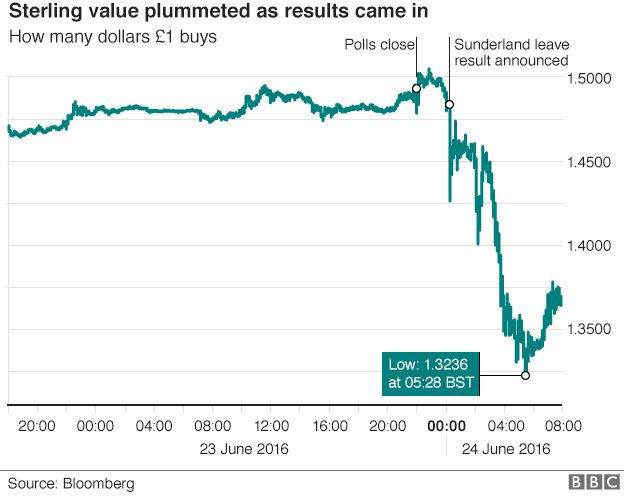
\includegraphics[width=0.8\textwidth]{sterling_plummet.png}
            \caption{Pound against the dollar around the result of the Brexit Vote \cite{bbc_news_2016}}
            \label{fig:sterling_plummet}
        \end{figure}

        To an extent, a trader can try to predict long term forex trends through following current events. For example, if a country is going through a period of political instability or uncertainty, a trader might choose to sell that currency. For example, the result of the 2016 "Brexit" vote caused the pound to fall to a 31 year low \cite{bbc_news_2016} \textit{(See Figure ~\ref{fig:sterling_plummet})}. This aspect of trading strategy presents challenges for algorithmic trading as it is difficult to inform a program about the political climate of a country. 



            \subsubsection{Mechanics of Trading}
            When trading forex, we talk about trading currency pairs \cite{hannah_2017}. A currency pair is represented in the form \textit{base currency/quote currency} and its value is how much of the quote currency the base currency buys. For example, EUR/USD = 1.2500 means that the Euro buys 1.25 US Dollars. When a pair is bought or sold, it involves buying ("going long") on one currency while simultaneously selling ("going short") on the other. E.g. putting a buy order on EUR/USD means going long on Euros while going short on Dollars.

            Every time a currency pair is traded on the forex market, its price changes. If the price rises in a certain time frame the market described as bullish, if it falls it is described as bearish. The goal of a forex trader is to to try predict these changes and  open buy or sell orders so that they can make a profit off the market movement when the order is closed. For example, if a trader thought that the price of EUR/USD was going to rise (the Euro strengthens against the dollar), they would buy EUR/USD. If the price of the Euro rises against the dollar, closing the trade at that point (selling the Euros) would result in an overall profit - the of Euros bought when closing the trade are more valuable than when the trade is opened, and so is worth more in whatever currency that the account is denominated in. If a downwards movement is predicted, then one can sell at the higher price and buy back at a lower price to make a profit.

            For day traders (the group for which this project is aimed at) one needs to open an account with a brokerage firm. An account is opened with a base currency - the currency with which is used to buy/sell assets and the currency which profits/losses are given in. To carry out trades, one deposits money into their account with the broker. Brokers can make money in a number of different ways, including putting commission on trades (which is discussed below) or buy offering services such as data analysis or advice for a monthly fee. 


            
            \subsubsection{Buying vs Selling}
            In trading, one does not have to previously own an asset to sell it. Shorting a currency works by borrowing the specified amount of the currency from your broker, agreeing to buy it back in the future at the future price. 
            
            Because of this, shorting has an inherent difference to buying in forex. When buying, you are betting on the price of a currency pair to rise. The worst outcome of a trade is that the value of your trade goes to 0 as the price of the pair does i.e. you lose all of your initial investment. When shorting, there is theoretically no limit on how much you could lose. The price of a currency pair can keep rising, and with it the amount you need to repay when closing the trade does \cite{russell}. In practice, the value of a pair will not keep rising to infinity, however, it is important to consider this when shorting.

            To protect against the danger of this, you can set a stop order when you start a trade. There are discussed more below.
                

            
            \subsubsection{Broker Fees}
            
            Broker fees can come in a number of different varieties. Disregarding fees a broker might charge for advice or other services, two common fee types are spread and commission \cite{tradimo_cost}.
            
            Spread is the difference between the buy and sell price of a currency pair quoted by a broker. This difference is given in pips - the fourth decimal place of a quoted price.\footnote{Imagine you are trading EUR/USD. The charts show a value of 1.2000 however your broker quotes two prices - a buy price of 1.2002 and a sell price of 1.2000. In this case we would say the spread is 2 pips. The small percentage on top of the actual value of the currency for the buy price is how the broker can make money off the spread.} Spreads can be fixed or variable depending on the broker. Variable spreads could depend on market volatility or trading volume for example - if a currency pair moves a large amount, a broker would prefer to set a larger spread. 

            Commission can come in fixed and variable forms as well. Fixed fee commissions tend to be very large, and targeted for people trading at high volumes. Variable fees are dependant on the volume traded, and so offer a good middle ground for all traders. Because of this, variable fees are growing in popularity \cite{llc_2016}. 



            \subsubsection{Trading on Leverage}
            As discussed above, currencies on the forex market do not move large amounts, and so huge investments are needed to make any non insignificant profits. To help with this individuals can trade with leverage from their broker. 
                        
            Trading on leverage is the act of borrowing money to boost the size of an investment. It acts as a multiplier on the original investment, increasing both the potential profits and losses from it. For example, if £100 worth of USD is bought with 50:1 leverage, the trade has a value of £5000. If the trade is closed when GBP/USD has moved up 20 pips, £10 is made instead of the £0.20 made if leverage is not used. \cite{lioudis_2018}This also works the opposite way however - if GBP/USD moves down 20 pips, then £10 is lost. Again, we can use stop orders to help protect against the risks of this. 



            \subsubsection{Stop Orders}
            Stop orders can be used by traders to decrease the chance of loss on a trade. Stop orders are instructions for a broker, telling them to close a certain trade when the market has reached a certain price. Stop orders can be used to both minimize losses and secure profits. e.g. if after buying a currency pair, the value starts to decrease, a stop order lower than the initial value can protect from the initial investment depreciating in value too much. On the other side, if a trader is buying a pair and is happy to "cash out" when they have made a certain amount off the market movement, they can set a stop order with a price higher than that bought, to protect from negative impact of potential future downward movements. Stop orders could be used for volatile markets, or on trades that won't be able to be appropriately monitored by the trader. \cite{momoh_2018}
            


            \subsubsection{"2\% Rule"}
            Stop orders can be used to help follow the 2\% rule - a strategy used to balance risk and reward in which a trader risks no more than 2\% of their available capital between all trades at any one time. When creating stop orders (and trading on leverage) one might use this to decide on the price to set the stop order at. \cite{staff_2017}



            
            \subsubsection{Open High Low Close}

            When, trading it can be useful to look at other meta data in addition to the raw exchange rate to inform what action to take. For example, if there is an indication that the market is very volatile at a point in time, one might wish to hold off on a trade as a prediction could be more likely to be false. 
            
            Open High Low Close data gives us some indication of the volatility of an asset during a particular time frame. Open/Close prices are the price of the asset at the start/end of the time period. High/Low are the greatest and smallest prices within a time frame. \cite{investopedia_OHLC}

            These charts are typically represented in two ways. The first is simple known as a "bar chart". It has two short horizontal dashes - one line pointing to the left (back in time) at the opening price and one line pointing to the right (forward in time) indicating closing price. The range (high/low) is given by a vertical line with one end at the highest price and another at the low \cite{barchart_OHLC}. \textit{(See Figure ~\ref{fig:barchart_ex})}

            \begin{figure}[h]
                \centering
                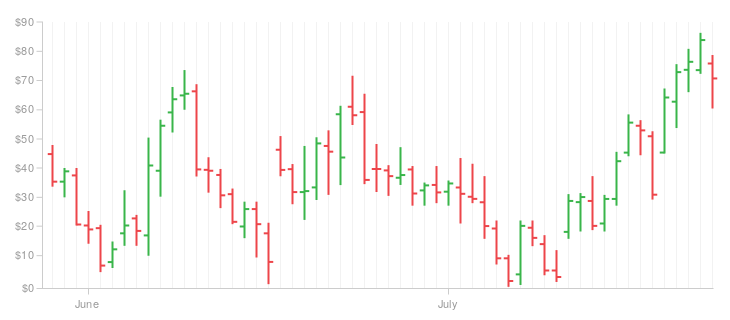
\includegraphics[width=0.8\textwidth]{OHLC_chart.png}
                \caption{Example of an OHLC Bar Chart \cite{barchart_OHLC}}
                \label{fig:barchart_ex}
            \end{figure}

            The other is known as a "Japanese Candlestick Chart" a thin vertical line represents the range, and a thicker vertical box represents the open and close price \cite{candlestick_OHLC}. \textit{(See Figure ~\ref{fig:candlestick_ex})} 

            \begin{figure}[h]
                \centering
                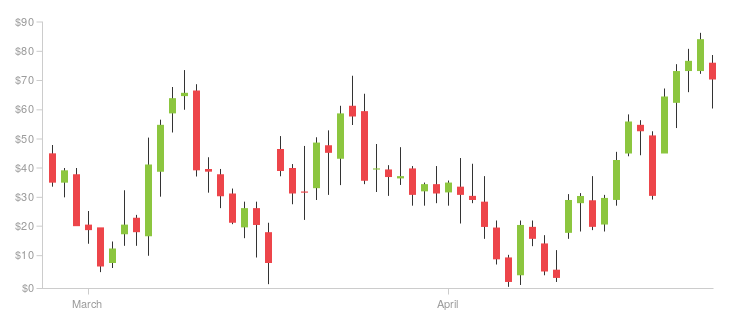
\includegraphics[width=0.8\textwidth]{candlestick_chart.png}
                \caption{Example of an OHLC Japanese Candlestick Chart \cite{candlestick_OHLC}}
                \label{fig:candlestick_ex}
            \end{figure}

            Both of these graphs (especially Japanese Candlestick) are usually colour-coded to help distinguish between bullish and bearish movements.
        


            \subsubsection{Why Trade Forex?}
            Forex trading attracts people for different reasons. One thing that makes forex attractive is that because movements are small, leverages offered are much larger than those on the stock market. This allows people to start trading effectively with relatively small sums of money. Unlike the stock market, forex is also open 24 hours a day (although retail brokers close on weekends - from 10pm Friday to 10pm Sunday UTC time).

            Others however might not trade forex with the intention of directly making money. If a trader was trading US stocks, they might be worried about the potential decline/volatility of the dollar. To offset this - allowing them to still make money off their stock trades overall, they could short USD against Euro\cite{investopedia_beginner}



    \section{Proposed Solution}

    The solution should be an aide to a day trader, giving short term (intraday) predictions in 15 minute intervals. It will take in data from previous prices in the market, and give some form of prediction of price movements for EUR/USD for a number of different points in the near future (e.g. 30 mins, 1 hour, 2 hours etc.). Neural networks will be used to make these predictions.

    The solution should include a web frontend that displays predictions along with measures of the accuracy of predictions in a graphical form to give users more information with which to make a judgement. This will include an API, with which a user should be able to get all data shown on the web page at a point in time in numerical form to be able to manipulate however they desire.

    Originally it was thought the solution would be one which carries out trades directly, however this was thought to be both too difficult as well as too limited - directly carrying out trades would require committing to a single api broker. In addition, it was thought that there would not be anyone who would be willing to use it as it would mean entrusting one's assets to a service that's out of they don't have much control of. 


            \subsection{End User}
            The target audience for the project is forex day traders using scalping/intraday strategies -  individuals carrying out short term trades at home who want to get a larger picture and be better informed before carrying out trades. 

            Such users might not have some of the more advanced analytical tools that a trader working in a hedgefund might have for example. Thus this could be a very useful tool for them.


    \section{Specification}
            
    \begin{enumerate}
        \item \textbf{Predictions} - see ~\ref{} for more details about 
        
        \begin{enumerate}
            \item All trained networks should be compared against specific, measurable critea on unseen test data in order to be able to be used in the final implementation. These criteria cannot be spcified at this point in time as it will be based off the final type of network being used, in order to be used in the final implementation (see ~\ref{sec:Measuring Success}).
            
            \item Predictions should be made for times at least 4 hours in the future.
            
            \item The networks must be able to take in real-time 15 minute data from the EUR/USD market from 10pm on Friday to 10pm on Sunday (UTC time).
            
            \item All predictions must be made within 30 seconds of receiving the real-time price data. 
            
            \item The recent accuracy of predictions should be able to be calculated in real time. The measure of accuracy again depends on the type of outputs the network gives and so this will be further elaborated on later in the document (see ~\ref{})
        
        \end{enumerate}

        \item \textbf{Webpage}
        
        \begin{enumerate}
            \item The webpage should display predictions of prices as well as previous price data graphically
            
            \item The webpage should display the recent accuracies of each network's predictions graphically
            
            \item The site should self-explanatory and relatively intuitive for a day trader to use, without too many specifics of its own. Any features and usage of the site should be explained in an "about page".
        \end{enumerate}

        \item \textbf{API}
        
        \begin{enumerate}
            \item Using an approved, random API key, a user should be able to retrieve all data of predictions and their accuracies numerically in an existing structured format which is easy to work with.
            
            \item A user should be able to request a unique API key with little resistance using only their email. A value entered that has already been used or that is an invalid email addresses will not get an API key
            
            \item The user's email should never be stored or sent in plaintext to maintain user privacy.

            \item API requests that are made too frequently should not be serviced
            
            \item If a user is inactive (makes no requests) for a month, their record will be removed
            
            \item All data of user requests should be stored.
            
            \item Daily metrics such as number of active of active users, total number of requests, number of requests that weren't serviced should be displayed to the console.
        
        \end{enumerate}


        
    \end{enumerate}

        \subsection{Justification}
        Justification of the specification points above are as follows 

        \begin{enumerate}
            \item \textbf{Predictions} 
            
            \begin{enumerate}
                \item Any predictions shown should be "useful" to some extent.

                \item 4 hours was thought to be a useful timeframe for day traders - it would fit with common trading timeframes. https://forextraininggroup.com/best-timeframes-trading-forex/
                
                \item Predictions should be shown for all open hours of the market (24/5).
                
                \item 30 seconds was thought to be an appropriate max processing time given the timescale of the predictions. This should also help ensure the server does not get overloaded during operation. The EUR/USD market was chosen as it is one of the most widely traded currency pairs and thus the potential user base for the project is large. In addition, this makes sourcing real-time and historic data easier.
                
                \item Given the random nature of the forex market, a network could provide better or worse predictions depending on the market behaviour at a certain point in time. Thus having some measure of recent accuracy could be useful to the user, and likely more so than the accuracy of the network on the test data used to assess the network using training.
            
            \end{enumerate}
    
            \item \textbf{Webpage} A website was chose for the frontend as it is more accessible being platform independent. Additionally most trading services such as brokers and sources of data use web pages so it would be a familiar format for users.
            
            \begin{enumerate}
                \item A graphical format is far easier and quicker to interpret that numerical data. This will allow users to get a feel for the predictions without getting bogged down in the specifics. Having the previous prices along with the predictions will also help users get a better sense of the predictions without having to change tab to look at price data separately.
                
                \item Displaying accuracies will allow the user to make a better judgement about the predictions. They should be shown graphically for the same reasons as those stated above.
                
                \item The barrier for entry for using the site specifically should be low in order not to deter users. The site should not require any technical knowledge beyond that needed for day trading.

            \end{enumerate}
    
            \item \textbf{API}
            
            \begin{enumerate}
                \item Returning data with an API allows the user more flexibility in how they wish to view/handle the predictions. An existing format should be used so that users will have experience/can easily find documentation for how to process the data they receive.
                
                \item Using an API key allows for authentication of a user - policing requests and ensuring the user is verified without much overhead.
                
                \item It is thought that the users will not need to be contacted, thus emails need not be stored in plaintext. To keep user privacy, emails should not be sent in plaintext either to reduce the impact of MITM attacks.  
    
                \item Not servicing requests made too frequently will help ensure good user etiquette and minimize server load.
                
                \item Removing inactive users will help reduce the amount of data stored making the API framework faster as querying the database for valid API keys will take as much time.
                
                \item In keeping a log of all API requests, metrics regarding the use of the API will be able to be calculated to get some insight into how users use the service and what they might need from the service in the future, aiding future development.
                
                \item Some of these simple metrics well help give a sense of the size of the client base and the usage over time.
            
            \end{enumerate}
        
        \end{enumerate}